\documentclass[11pt]{article}
\usepackage[margin=0.88in]{geometry}
\usepackage{fontspec}
\setmainfont{lmroman10-regular.otf}[BoldFont=lmroman10-bold.otf,ItalicFont=lmroman10-italic.otf,BoldItalicFont=lmroman10-bolditalic.otf]
\setsansfont{lmsans10-regular.otf}[BoldFont=lmsans10-bold.otf,ItalicFont=lmsans10-oblique.otf,BoldItalicFont=lmsans10-boldoblique.otf]
\setmonofont{lmmono10-regular.otf}[Scale=0.87]
\usepackage{amsmath,amssymb,booktabs,xcolor,hyperref}
\usepackage{unicode-math,xurl,pgfplots}
\pgfplotsset{compat=1.17}
\setmathfont{latinmodern-math.otf}
\definecolor{ink}{RGB}{28,65,86}
\hypersetup{colorlinks=true,urlcolor=ink,linkcolor=ink,citecolor=ink}
\setlength{\parindent}{0pt}
\setlength{\parskip}{5pt}
\raggedbottom
\newcommand{\head}[1]{{\small\bfseries\color{ink} #1}\par}
\begin{document}
\head{RESEARCH NOTEBOOK \hfill 27 NOVEMBER 2026}
{\LARGE\bfseries Can one incomplete computation change the next?}\par
\section*{The first decision}
A model can generate different answers to a puzzle and still gain nothing from their differences. In the fork's earlier Sudoku study, two digit-conditioned paths reached one extra board, lost another, and both proposed digits were wrong on the extra solve. That makes a branch label a poor explanation of the recovery. Our primary interest is behavior: does a fresh intermediate result let the model compute something useful on a combination it has never trained on?
\par
\textbf{Worked case.} The visible tables are $F=(2,0,3,1)$ and $G=(1,3,0,2)$, indexed from zero. For query 0, the useful intermediate is $F(0)=2$. Reading row 2 of $G$ yields 0. Always copying the query happens to work here. Change only the second table to $(3,1,2,0)$. The same intermediate now produces 2, and copying fails. Demonstrations and query arrive together. Holding back a clue would change the problem.
\par
\textbf{Cheapest explanation.} A single four-valued scratch register and two indexed reads solve every input exactly. The first experiment asks a narrower question. Given the same dense recurrent model and two updates, is sending an updated peer state better than sending the peer's original encoding? Each slot sees everything. A positive result can identify a benefit of a pathway under this training regime. It cannot establish that either slot represents a belief.
\par
\textbf{What changed our choice.} Conditional proof by cases has a direct constraint-programming ancestor. A dense recurrent parent can exactly implement two communicating slots. Both observations argue for measuring a rival before spending cluster time. We registered a paired CPU study and a separate fixed-bank check on the public training tasks of ARC-AGI-1. A learned single-register reader tests whether a small architectural prior already solves the diagnostic.
\par
\textbf{What we learned.} Across three seeds, fresh messages scored 95.02\% and stale messages 96.29\% on unseen table pairs. In the two-world follow-up both architectures solved all 4,608 primary queries per seed. Inspecting the alternatives explained the tie: the selector always had both possible answers on offer. On real ARC grids the fixed bank solved 11 of 400 public training tasks. Every success used one factor alone.
\par
\textbf{Decision.} Close the claim that these designs earn more training on these tasks. The original question remains open. Before funding a new architecture, require a natural input on which a legal intermediate changes a subsequent operation and the correct answer lies outside the pre-message candidates.

\par
\textbf{Fresh Sudoku result, 28 November.} A peer correction changed the next prediction on 35 boards, but aligned, shuffled and untouched continuations solved the same 163/256. Serial reasoning solved 166. Two boards were recovered after both branch endpoints failed; both also recovered with the peer correction disabled. Park this write and its proposed training run.

\newpage
\section*{Two rounds of computation}
Let $x\in\{0,1\}^{36}$ concatenate the eight one-hot four-symbol rows of $F,G$ and the one-hot query. For slot $k\in\{1,2\}$ let $h^0_k=\tanh(E_kx+b_k)\in\mathbb R^{32}$. The encoders $E_k\in\mathbb R^{32\times36}$ and biases $b_k$ identify the two slots. With peer $j=3-k$, both slots update in parallel:
\[
h^{t+1}_k=\tanh(Uh_k^t+V m_j^t+b),\qquad t=0,1.
\]
Here $U,V$ are shared $32\times32$ matrices and $b$ has 32 entries. The live arm uses $m_j^t=h_j^t$; the static arm uses $m_j^t=h_j^0$. Only the second round differs. A learned four-way classifier reads both final states. All examples supply both complete tables. Only the final answer is supervised. There are no branch labels, conditional masks or access selectors.
\par
\textbf{Training.} Draw an ordered pair of permutations and query from the training groups; run the two encoders and both rounds; compute categorical loss on the final answer; update all parameters. Initial weights and the example stream are paired across arms. Repeat for each of three seeds. \textbf{Inference.} Encode one input, run both parallel updates twice, and return the label-free argmax. To intervene, substitute the first encoder state for the fresh message only at round two. Each branch continues to update. Training a static model from scratch helps interpret damage from an unexpected inference-time substitution.
\par
\textbf{Exact reduction.} Stack $h_1^t,h_2^t$ into a 64-vector. One dense recurrent map with blocks $[U,V;V,U]$, elementwise $\tanh$ and repeated bias produces the identical live update. Induction from the same initial states proves equality for all rounds and inputs. This leaves sample efficiency and optimization open. Width, clock time and the availability of role-specific encoders must be reported.
\par
\textbf{A stronger single trajectory.} Let $T_i\in\{0,1\}^{4\times4}$ give one-hot output rows for table $i$, $s\in\Delta^3$ the current symbol distribution. A shared learned address matrix $A\in\mathbb R^{4\times4}$ maps $s$ to four row probabilities $p=s\,\mathrm{softmax}_{\rm row}(A)$. Step $t$ has learned table probabilities $w_t\in\Delta^1$. Update $s\gets \sum_i w_{ti}pT_i$, starting from the query. Predict the most likely final symbol. Only the endpoint trains the address and routing logits. This model spends its prior on indexing and reuses the same reader twice. Multi-hop memory networks already use this principle \cite{mem}.
\newpage
\section*{What would change the decision?}
\textbf{Primary prediction, registered at 71a689d.} On unseen ordered table pairs with nonidentity second operation, a fresh peer message should increase exact query accuracy over an independently trained stale-peer model because the second update can condition on the intermediate. There are 24 permutations. Within each second table, reserve four first tables for development, four for a locked characterization partition and sixteen for training. Keep the four queries for a pair together. The primary development set has 92 groups and 368 queries. There are four identity-second-table groups. This small negative control asks whether any advantage persists when one lookup suffices.
\par
\textbf{Stopping rule.} Require at least five percentage points of mean gain, a positive gain for all three training seeds, a positive lower paired group-bootstrap bound, and a drop under the stale-message intervention. Match examples, updates, initial conditions, width and arithmetic. Extend both arms together if the registered training-curve rule fires. Report grouped task uncertainty separately from the three seed differences. A missed gate parks this mechanism at this budget. The diagnostic has no pre-message branch answer heads, so it cannot establish success beyond selecting pre-message answers.
\par
\textbf{Two discarded shortcuts in the argument.} In the seed memo, if answer vectors $b_k$ are fixed and a parent merely accumulates $\sum_k(w^{t+1}_k-w^t_k)b_k$, summing over $t$ cancels intermediate weights. The entire write equals $\sum_k(w^T_k-w^0_k)b_k$. A nonlinear parent that uses the message to select a new operation escapes this algebraic reduction, but a single recurrent parent may still learn the same function. The memo's toy accuracy was author-reported; it did not guide model selection here.
\par
A second design splits a variable into exhaustive cases, infers consequences independently, and returns their common implications. For example, $u=x$, $v=1-x$ imply $u\lor v=1$ under either binary value of $x$. An unresolved case can thereby determine a later lookup. Constructive disjunction already unions supported domains across cases \cite{cc}. With two scalar branch scores even $\max(a,b)=(a+b+|a-b|)/2$. Max fusion alone cannot distinguish proof by cases from an ordinary mean-and-disagreement feature. We deferred training this design.
\par
\textbf{Peer review record.} Independent proposals emphasized case analysis and role binding. The former's architect then challenged the latter: for geometry $g$ and a global recoloring $c$, $g(c(X))=c(g(X))$; successful recombination may reflect fixed roles. The literature reviewer independently identified multi-hop reads as a serious rival. Generalizing across held-out tables cannot identify semantic roles. A more specific future intervention would swap sender states across inputs sharing exactly one factor, check donor-consistent predictions, and include a same-factor placebo.
\newpage
\section*{Fresh peer messages changed predictions}
\begin{center}
\begin{tabular}{rrrrrrr}
\toprule
Seed & Fresh & Static & Gained & Lost & Stale clamp & Serial reader\\
\midrule
31 & 351 & 344 & 22 & 15 & 198 & 251\\
47 & 358 & 357 & 9 & 8 & 198 & 277\\
83 & 340 & 362 & 4 & 26 & 152 & 368\\
\bottomrule
\end{tabular}
\end{center}
Counts are correct queries out of the same 368. Gained and lost compare separately trained fresh and static models on paired inputs. The mean fresh-minus-static difference was $-1.27$ percentage points. The 95\% interval from 2,000 draws of 92 operation pairs was $[-2.81,+0.27]$ points conditional on the three training seeds. All six dense models fit training exactly; none triggered the extension. Static reached 96.29\%, leaving less than the registered five-point margin even for a perfect challenger. The identity-second-table control had fresh/static scores of 16/15, 16/16 and 15/16 out of 16.
\par
\textbf{One changed prediction.} For seed 31, query 2, $F=(2,1,0,3)$ and $G=(0,3,1,2)$, the correct answer was 0. The fresh model returned 1. Both clamping and the separately trained static model returned 0. Conversely, one fresh-only gain survived clamping. Intervening on a learned wire and retraining without the wire answer different questions.
\par
\textbf{What the donor could transmit.} For each seed, 100 inputs had matched eligible donors. Active message transplants produced the donor target 39, 44 and 53 times; placebo transplants preserved the original prediction 93, 92 and 89 times. With $G,q$ fixed and $G$ bijective, the correct intermediate uniquely identifies the final answer and vice versa. This design cannot distinguish a message carrying $F(q)$ from one carrying $G(F(q))$.
\par
\textbf{Optimization and cost.} A 20-parameter two-read model acquired the intended table order in all seeds. Only seed 83 acquired the identity address map and solved all queries. The other two suppressed the correct address and reached 251 and 277. The deterministic table follower solved every case. These results distinguish an available algorithm from its reliable acquisition. Both dense arms used 4,708 parameters and 10,752 dense multiply-accumulates per query. The serial reader used 112 multiplications in its matrix reads and mixtures. Latencies include framework dispatch. PH1 used NumPy, the reader used PyTorch; neither implementation sets a hardware lower bound.
\par
\begin{center}
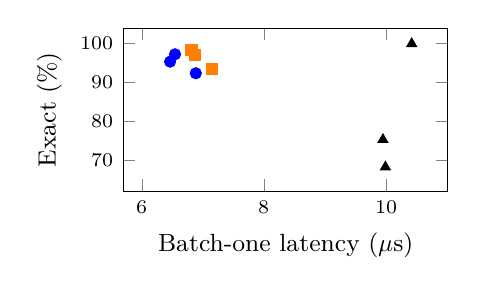
\begin{tikzpicture}
\begin{axis}[width=.47\linewidth,height=3.65cm,xlabel={Batch-one latency ($\mu$s)},ylabel={Exact (\%)},xmin=5.7,xmax=11,ymin=62,ymax=104,tick label style={font=\scriptsize},label style={font=\small}]
\addplot[only marks,mark=*,blue] coordinates {(6.46,95.38)(6.54,97.28)(6.88,92.39)};
\addplot[only marks,mark=square*,orange] coordinates {(7.14,93.48)(6.87,97.01)(6.81,98.37)};
\addplot[only marks,mark=triangle*,black] coordinates {(9.98,68.21)(9.94,75.27)(10.41,100)};
\end{axis}
\end{tikzpicture}
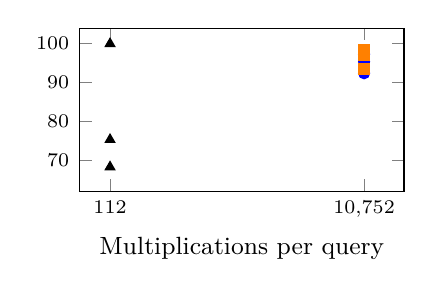
\begin{tikzpicture}
\begin{semilogxaxis}[width=.47\linewidth,height=3.65cm,xlabel={Multiplications per query},xmin=65,xmax=22000,ymin=62,ymax=104,xtick={112,10752},xticklabels={112,{10,752}},tick label style={font=\scriptsize},label style={font=\small}]
\addplot[only marks,mark=*,blue] coordinates {(10752,95.38)(10752,97.28)(10752,92.39)};
\addplot[only marks,mark=square*,orange] coordinates {(10752,93.48)(10752,97.01)(10752,98.37)};
\addplot[only marks,mark=triangle*,black] coordinates {(112,68.21)(112,75.27)(112,100)};
\end{semilogxaxis}
\end{tikzpicture}\\[-2pt]
{\small Circles: fresh. Squares: static. Triangles: serial. Each point is one seed.}
\end{center}

\newpage
\section*{Two conditional worlds and a fresh lookup}
PH1 supplied a composition with a unique intermediate. To instantiate alternatives, the follow-up supplies two equally admissible worlds, $A$ and $B$. Each contains a four-row symbol permutation. Read the same query $q$ under each assumption. If the resulting symbols have equal parity, return the second entry of a visible two-entry answer table $R$; otherwise return the first. For $A=(2,0,3,1)$, $B=(0,2,1,3)$, $q=0$ and $R=(3,1)$, the reads give 2 and 0. Both are even, so return 1. Changing only $B(0)$ to an odd symbol selects 3. The two worlds, their boundaries and the downstream lookup are supplied. The parity relation is learned from final answers.
\par
\textbf{Execute under each assumption.} For each world, use a shared learned $4\times4$ row-address matrix (softmax over the row for $q$), multiply by the visible four-row one-hot table, then read from a learned $4\times8$ symbol embedding. Denote the two resulting eight-vectors by $a,b$. Form a 16-vector $v=[a+b;a\odot b]$. A 16-unit tanh layer and sigmoid readout give $w\in[0,1]$. The joint model returns the argmax of $(1-w)R_0+wR_1$ with each entry encoded as a four-way one-hot vector. Its selector rival uses the same network for $w$ and two local scalar addresses $u_A,u_B$ from shared affine symbol reads with independent role biases. Its final address is $(1-w)u_A+wu_B$. Both arms minimize negative log probability of the final answer by differentiating through the reads. Only supplied tables and query enter inference.
\par
\textbf{Decision experiment.} Group by unordered world pair before generating both orders, queries and answer tables. Train on 200 groups, develop on 50, reserve 50 unexamined. Three matched seeds, 1,200 steps, batches of 128. Compare on nonconstant answer tables where the choice matters. The negative control has identical answer entries and is solved structurally. The fixed training-accuracy extension did not fire.
\par
\textbf{Result.} Each model solved 4,608/4,608 primary and 1,536/1,536 negative-control rows in every seed. Gains and losses were both zero on all 50 development groups. The empirical paired bootstrap degenerates at zero; this measures no general-population equivalence margin. In every primary row, for all seeds, the first hard branch proposal was $R_0$ and the second $R_1$. The chooser performed the entire relational decision. The observation required to support an advantage for constructing a new answer never occurred.
\par
\textbf{Adversarial re-review.} On 3,456 eligible rows per seed, replacing the second world state by one from an opposite-parity donor switched every prediction; every same-parity placebo preserved it. Because donor and recipient share $A,q,R$, the patched model exactly reproduces the intact donor computation. This verifies the isolated pathway. It cannot identify an invented hypothesis or a changed downstream operation. Executing the two reads serially produced exactly the same probabilities in float32 (maximum absolute difference zero). The join used 337 parameters; selection used 347. For the join, batch-one vectorized reads took 13.3--14.7 $\mu$s versus 19.4--20.0 $\mu$s serially on one CPU thread. This is a dispatch saving on this implementation. Both schedules spend the same logical work. Close the new-answer claim on this task.

\par
Across all six PH2 models, training took 0.22--0.31 seconds per arm on this machine. A separate complete rerun used 309 MB peak process RSS and reproduced the saved predictions byte for byte. PH1 training took 0.15--0.16 seconds per arm with 45 MB peak process RSS for the campaign. The hardware and runtime differ from a GPU application benchmark.

\newpage
\section*{Evidence and application boundary}
\textbf{Inherited.} The native model retained every reached exact answer through macro depth 16 in the earlier development record. At matched work, early Gaussian branching reached 123 versus 143 boards and late branching reached 161 versus 162. Learned digit conditioning tied the serial comparator at 162. These are archived results on 256 boards, not replications in this study. The old 896-board holdout remains sealed.
\par
\textbf{Application benchmark.} Use public ARC-AGI-1 training tasks only. Before scoring, fix a bank of eight geometric transformations and fit one global pointwise colour table to all visible demonstrations. Predict once per query, counting abstentions as failures. Compare with leave-one-demonstration-out reranking and charge the extra fits. Measure exactness over whole original tasks. The hand-built bank quantifies a real shortcut on natural grids. The neural table experiment learns from endpoint labels on a different interface; transfer remains untested.
\par
\textbf{Infrastructure.} The branch began at \texttt{2de6e27}. PH1, PH2 and the ARC fixed bank used local CPU. A GH200 verification replay and fresh-puzzle intervention used 32 and 131 allocated seconds respectively. No current GPU commitment. The sealed Sudoku and ARC evaluation sets remain outside these experiments.
\par
\textbf{Measured.} Twelve of the 400 original tasks admitted an exact fit on all demonstrations. Eleven solved every query (2.75\%; descriptive Wilson interval 1.54--4.86\%). Reranking changed zero decisions. Seven solved tasks used geometry alone and four recoloring alone. Across all 400, the mean within-task fraction of withheld demonstrations predicted correctly was 2.56\%. The successful set contains no selected program needing both factors.
\par
\textbf{A failed fit.} In training task \texttt{aabf363d}, the large region took the singleton's colour and the singleton disappeared. A global colour map fit both demonstrations perfectly. It failed on 16 of the 49 query cells when colour 8 appeared in the large region. This motivates investigating object roles, but choosing a new neural architecture on this example would make it discovery data. Fresh evaluation would be necessary.
\par
\textbf{What stays open.} The constructed interfaces expose discrete tables and role boundaries. A grid or text system would need to learn which cells or tokens constitute a hypothesis, identify a legally observable consequence, and select a later operation using it. Neither CPU study implements this transfer. Neither consumes the old Sudoku holdout or the ARC evaluation tasks.
\par
\begin{tabular}{@{}p{.23\linewidth}p{.71\linewidth}@{}}
\toprule
Evidence status & Decision on 27 November 2026\\\midrule
Inherited & Native stability and branch-oracle counts motivated testing content.\\
Verified here & Fresh messaging missed its gate; selection covered all PH2 answers.\\
Hypothesis & Two incomplete paths may jointly supply a useful future argument on real inputs.\\
Open question & Can learned branch-local consequences change an unconstrained next operation on a natural task where selection fails?\\\bottomrule
\end{tabular}

\newpage
\section*{Do wrong Sudoku branches contain different useful digits?}
For a communication mechanism to help, the sending branch must contribute something the receiving branch lacks. Sudoku offers a simple first test because the same puzzle has one target grid. At a fixed blank the archived model proposed two digits. Each proposal edited the working state and ran the native model twice. Even when both predicted grids were wrong, one might supply correct digits where the other was wrong.
\par
\textbf{Which boards qualify?} In the historical 256-board development cohort, 94 boards had two wrong branch endpoints. On 77 the endpoints differed. On 76 of those, none of the candidates from the matched serial continuation was exact. These 76 boards were chosen from archived GH200 correctness flags before inspecting per-cell results. The archive did not store the full digit grids. We recovered the native checkpoint and the learned edit, checked their SHA-256 hashes and replayed the 76 boards on CPU from the saved depth-two development states. Reconstruct the depth-12 state and rerun both conditional paths and four more unconditioned serial steps. CPU and GPU numerical differences can change an ambiguous fork; we report replay eligibility separately.
\par
\textbf{How to read the ceiling.} Let $a_i,b_i$ be the two endpoint digit predictions and $y_i$ the true digit at cell $i$. A label-aware chooser can assemble the exact solution from those two grids if and only if every cell satisfies $a_i=y_i$ or $b_i=y_i$. A single shared error disproves sufficiency for that board. Reciprocal contributions require at least one cell correct only in A and at least one correct only in B. These are retrospective diagnostics; labels never choose digits in a deployed model. Averaging the endpoint logits supplies a separate label-free check.
\par
\textbf{CPU replay.} Of the 76 archived cases, 50 still had two different, wrong endpoints and a serial miss on CPU. The selected blank and proposed pair of digits matched the archived values on 1/76 boards. On 14/50 replay-eligible boards, each branch was correct on at least one cell missed by the other. A chooser with access to the true digits could assemble 0/50 exact boards. The median number of cells wrong in both endpoints was 30. Averaging the endpoint logits solved 0/50 boards. These counts apply to the selected failures. They do not estimate full-cohort improvement.
Of all 76, averaging solved five, but each of those already had an exact CPU branch endpoint. Agreement on only one selected blank-and-digit pair prevents attribution to the historical GH200 trajectories. Numerical divergence is a possible explanation; the cause has not been established.
\par
\textbf{Verified on the original runtime.} Slurm job 8930277 reproduced all 76 fingerprints, including the chosen cell, proposed digits, four branch digit readouts and stepwise exact flags. Each branch supplied at least one correct digit missed by its peer on 17/76 boards. Across the 76 failures the median shared-error count was 29. No target could be assembled from the two grids, and average logits solved none. These fingerprints are stronger than matching aggregate totals, but the archive has no original complete grids for a bitwise comparison. The job completed on one GH200 in 32 seconds (0.0089 GPU-hours). The full new predictions are retained on project storage.

\par
\textbf{Registered follow-up.} On fresh original puzzles, freeze both branches and their continuation. At a fixed step deliver the peer's correction to corresponding disagreement cells. Compare with the same vectors permuted among the same cells, and with the untouched parent. Equalize observations, total block calls, and post-cast correction size. Choose sites without labels. Report paired exact gains and losses over all puzzles and inspect which later computation changes. The independent reviewer emphasized that damaging the shuffled arm is insufficient: aligned communication must improve the unmodified trajectory too. Compare a serial solver and an online whole-trajectory selector before training. The following page reports the outcome.

\newpage
\section*{Which existing result could explain a win?}
\textbf{Learned read, then read again.} End-to-End Memory Networks (Section 2) combine a weighted read with the query and use it for the next hop. A single register is sufficient for our tables. Recurrent Independent Mechanisms already maintain multiple private states and learn when to communicate. The algebra on page 2 places the present fresh arm inside the model class of a tied block-recurrent network. A wiring diagram alone provides no novelty. \cite{mem,rims}
\par
\textbf{Reweight, select or synthesize.} Multiplex Thinking samples several token embeddings, merges them and takes another LM step. GRAM (Sections 2.1--2.3) draws recursive stochastic latents from an inference prior and can apply a scorer or voting across trajectories. Guided Reasoning (Sections 4.1--4.3) resamples particles online using a learned stopping head. Both offline selection and online allocation are relevant controls. On ARC, Latent Program Networks (Sections 4.1--4.3) fit a shared latent program to observed demonstrations by sampling or optimization; charge their program evaluations and gradients. \cite{multiplex,gram,guided,lpn}
\par
\textbf{Native capability comparisons.} TRM's released implementation carries answer and workspace states; its stock evaluation forces the configured maximum depth. The ARC evaluator also uses puzzle identifiers and augmented predictions. FPRM means Fixed-Point Reasoning Model; its release uses the name FPTRM and a damped fixed-point update with convergence-based stopping. InfiLoop aggregates history within a single trajectory. Its public Sudoku solver retries surviving boards from scratch at different depths and checks a legal puzzle certificate. An equal-depth run and a native solver run answer different questions. SE-RRM supplies symbol equivariance. Its Sudoku Table 2 varies the number of supervision steps; Section 3.2 describes its ARC demonstration exposure. \cite{trm,fprm,infi,se}
\par
These releases have different task interfaces, conditioning, stopping and selection costs. None is a four-symbol PH1 or PH2 checkpoint. The ARC bridge used a fixed untrained program on the public training set; comparing its 2.75\% to an ARC evaluation-set headline would be invalid. We ran no released checkpoint in this revision. Before any natural benchmark claim, train or run the strongest compatible models at their native settings and with common legal information, report their costs, and include a trained single-trajectory rival. The accompanying \texttt{prior-art.md} records source sections, checkpoint paths, reviewer discussion and access limitations.
\par
\textbf{Resource decision.} Retire these two performance claims at the tested budgets. A repeat of the conditional diagnostic on one GH200 is technically prepared (15 minute wall limit, at most 0.25 requested GPU-hours); it would measure GPU dispatch and numerical parity only. The recommended allocation is zero. A future study needs an open answer space and a genuine future operation that can be causally changed by complementary consequences. No cluster job or spending commitment is pending.

\newpage
\bibliographystyle{plain}
\bibliography{references}
\end{document}
